After we saw the intuition of why we need NNs, what they roughly are, and some example applications, we'll now take a look at what an Artificial NN really is.
\begin{itemize}
  \item Generally speaking, it is a computing system inspired by, but not identical to, biological NNs. 
  \begin{note}
  \begin{itemize}
    \item Since there are many differences between real NNs and artificial ones, the terms are sometimes criticized.
  \end{itemize}  
  \end{note}
  \item It learns to perform tasks by considering examples without being explicitly programmed.
  \item Artificial NNs are collections of connected artificial neurons. 
  \begin{note}
    \begin{itemize}
      \item The connections correspond to weights that can be updated to make the error on the training data smaller.
    \end{itemize}  
  \end{note}
\end{itemize}

\subsection{Historical background}
Throughout the history of developing NNs (see \ref{fig:6_bg_history}), we can see two paradigms for AI:
\begin{enumerate}
  \item Logic-inspired based on \textbf{reasoning} \begin{note}\footnotesize"Good old-fashioned AI"\end{note}
  \begin{itemize}
    \item Symbolic rules over symbolic expressions
    \item Programmed using unambiguous language
    \item[$\rightsquigarrow$] $1943 - 2005\!:$ beat NNs with various other methods
  \end{itemize}
  \item Biologically-inspired based on \textbf{learning}
  \begin{itemize}
    \item Large vectors representing neural activities
    \item Vectors learned from data
    \item[$\rightsquigarrow$] $2005-2010\!:$ NNs show more promising results (improvements in backpropagation, more training material, computational power)
    \item[$\rightsquigarrow$] $>\!2010\!:$ major investments \begin{note}\footnotesize(Google, IBM, Apple etc. for Alexa, Siri, autonomous driving, ...)\end{note}
    \item[$\rightsquigarrow$] $>\!2018\!:$ high on political agenda
  \end{itemize}
\end{enumerate}

\begin{figure}[H]
  \centering
  \begin{subfigure}{\textwidth}
    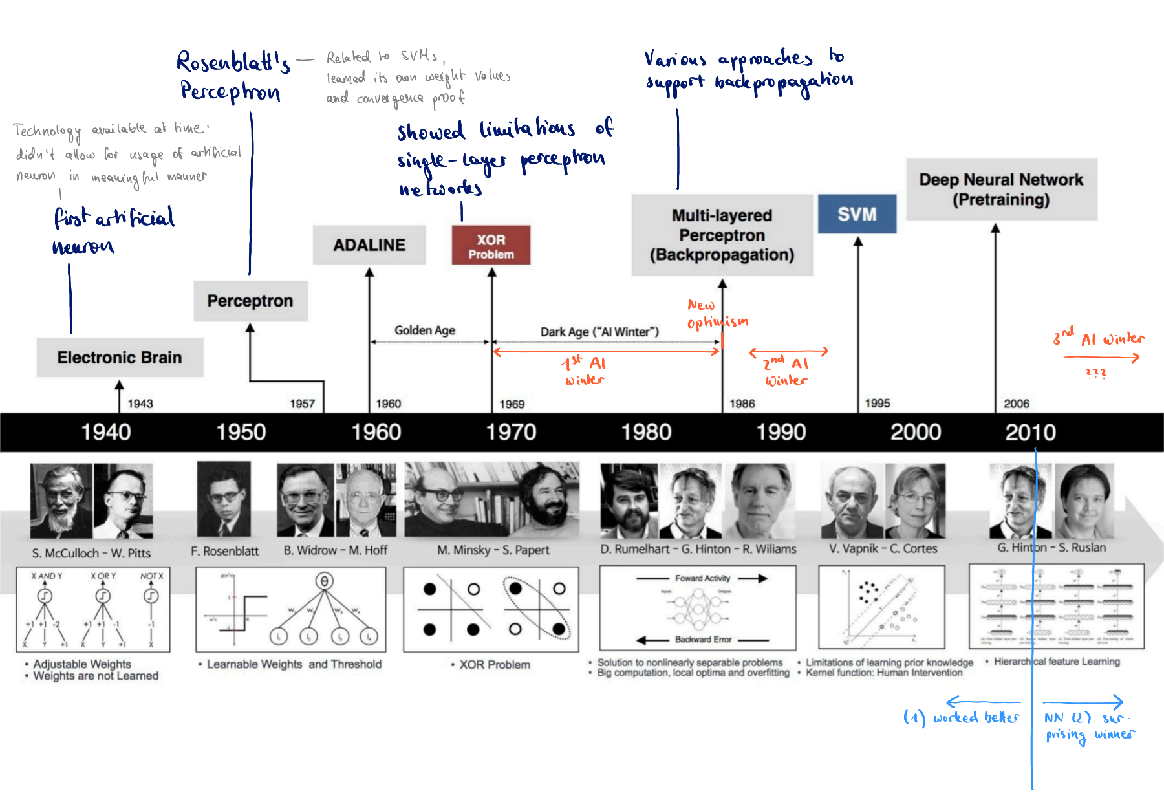
\includegraphics[width=\textwidth]{assets/nn/bg__history.pdf}
  \end{subfigure}
  \caption{History of Neural Networks}
  \label{fig:6_bg_history}
\end{figure}

In 2018, the Turing Award was given for the development of a convolutional NN, concretely the conceptual and engineering breakthroughs making deep neural networks a critical component of computing. Still, for a NN to work successfully, a lot of engineering and trial-and-error is necessary.
\begin{itemize}
  \item The main advantages of ANNs:\sidenote{Pro and Con of NNs}
  \begin{itemize}
    \item NNs are best at identifying patterns or trends, so they are well suited for:
    \begin{itemize}
      \item Sales forecasting, logistics, customer behavior, security, medicine
      \item Specific tasks: face recognition, traffic sign classification, sentiment analysis, diagnosis of hepatitis, speech recognition, hand-written text recognition, computer vision, pattern recognition, etc.
    \end{itemize}
    \item Can model complex (non-linear) functions
    \item Generic and flexible, driven by data
    \item Good performance on unseen noisy data
    \item Can handle images, sound, text, video, etc.
    \item After the model is learned: can be applied fast
  \end{itemize}
  \item Main disadvantages:
  \begin{itemize}
    \item Only works with lots of training examples
    \item Time- and resource-consuming
    \item Non-transparent (black-box, interpretation of hidden layers is difficult $\rightarrow$ keyword explainable AI)
    \begin{itemize}
      \item What the Hidden layers are doing is feature extraction. However due to the nonlinearity, it can be hard to interpret what feature they're extracting,
    \end{itemize}
    \item Risk of overfitting
    \begin{itemize}
      \item Large number of parameters allows more complex functions (with enough parameters, you can fit any data set exactly)
      \item But they require lots of training data and are drawn to overfitting the model
      \item So they "learn" the training data by heart, without abstracting
    \end{itemize}
    \item Performs worse on well-defined problems
    \item Can be "hacked" (add noise, switch one pixel $\rightarrow$ wrong classification, etc.)
  \end{itemize}
\end{itemize}

\subsection{Human and Artificial Neurons}
Now that we know some of the historical developments, we'll take a look at how the ideas to develop artificial NNs came up.

The "original" biological inspiration is the \textbf{Human brain} with around 100 billion neurons. The human brain learns in the way displayed in \ref{fig:6_bg_bio_neuron}.

\begin{figure}[H]
  \centering
  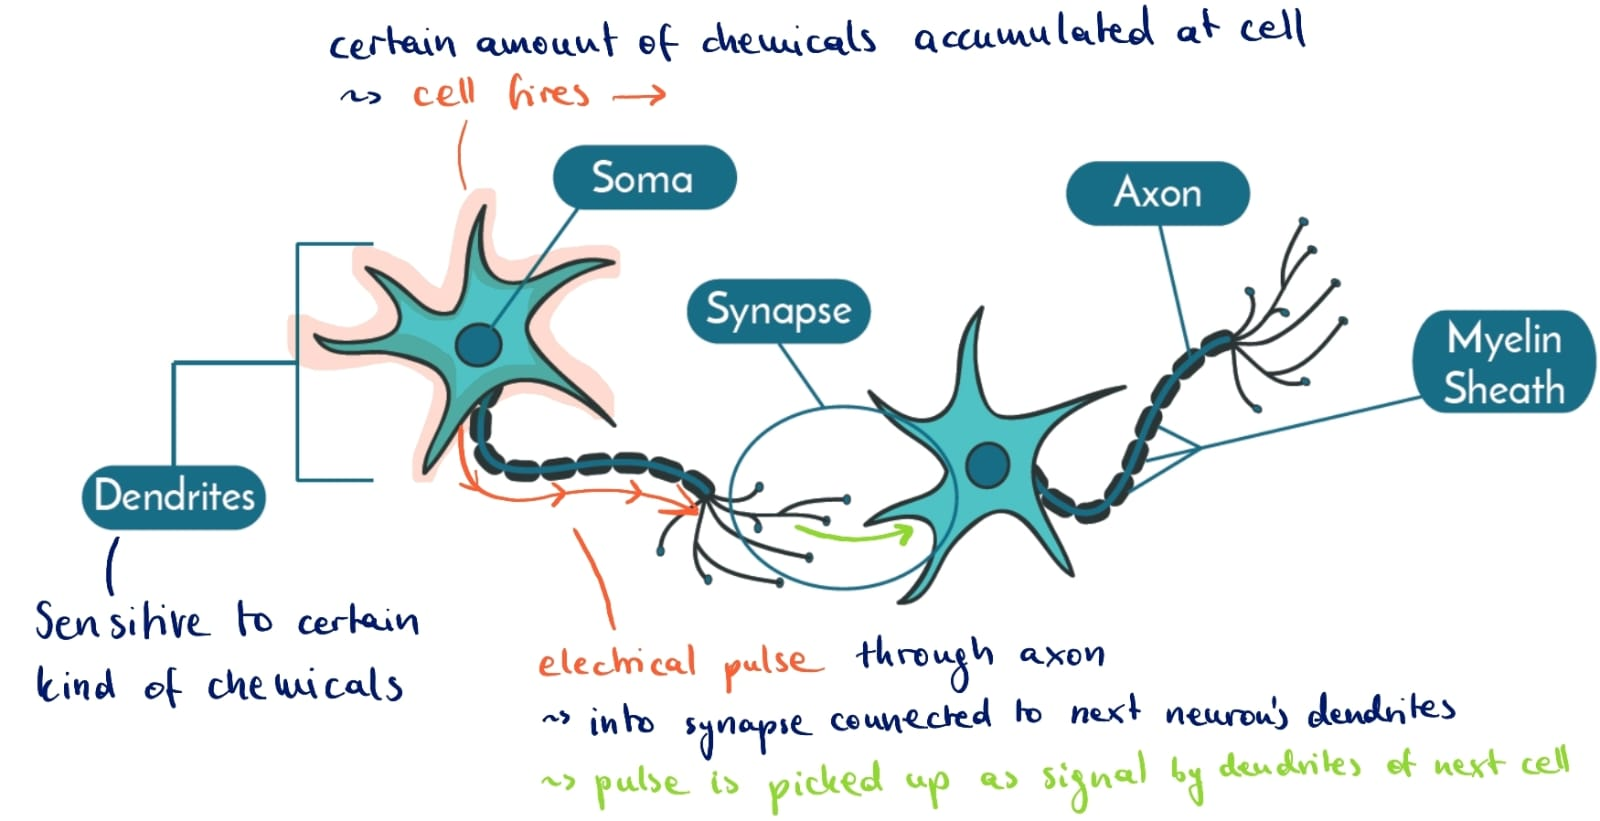
\includegraphics[width=0.7\textwidth]{assets/nn/bg__bio_neuron.png}
  \caption{Biological neuron (learning)}
  \label{fig:6_bg_bio_neuron}
\end{figure}

So on a more abstract level: when a neuron receives excitatory input, learning occurs.
\begin{itemize}
  \item The input needs to be sufficiently large compared to its inhibitory input, only then is a spike of electrical activity sent down the axon.
  \item Learning is then the change of the effectiveness of the synapses, and/or the influence of one neuron on other changes.
\end{itemize}

This abstraction can be reduced to this simple (artificial) neuron shown in \ref{fig:6_bg_simple_an}. This is also known as a \textbf{single-layer perceptron}\sidenote{Single-layer/Rosenblatt's perceptron} which is the simplest feedforward neural network and only works for binary classification.

\begin{figure}[H]
  \centering
  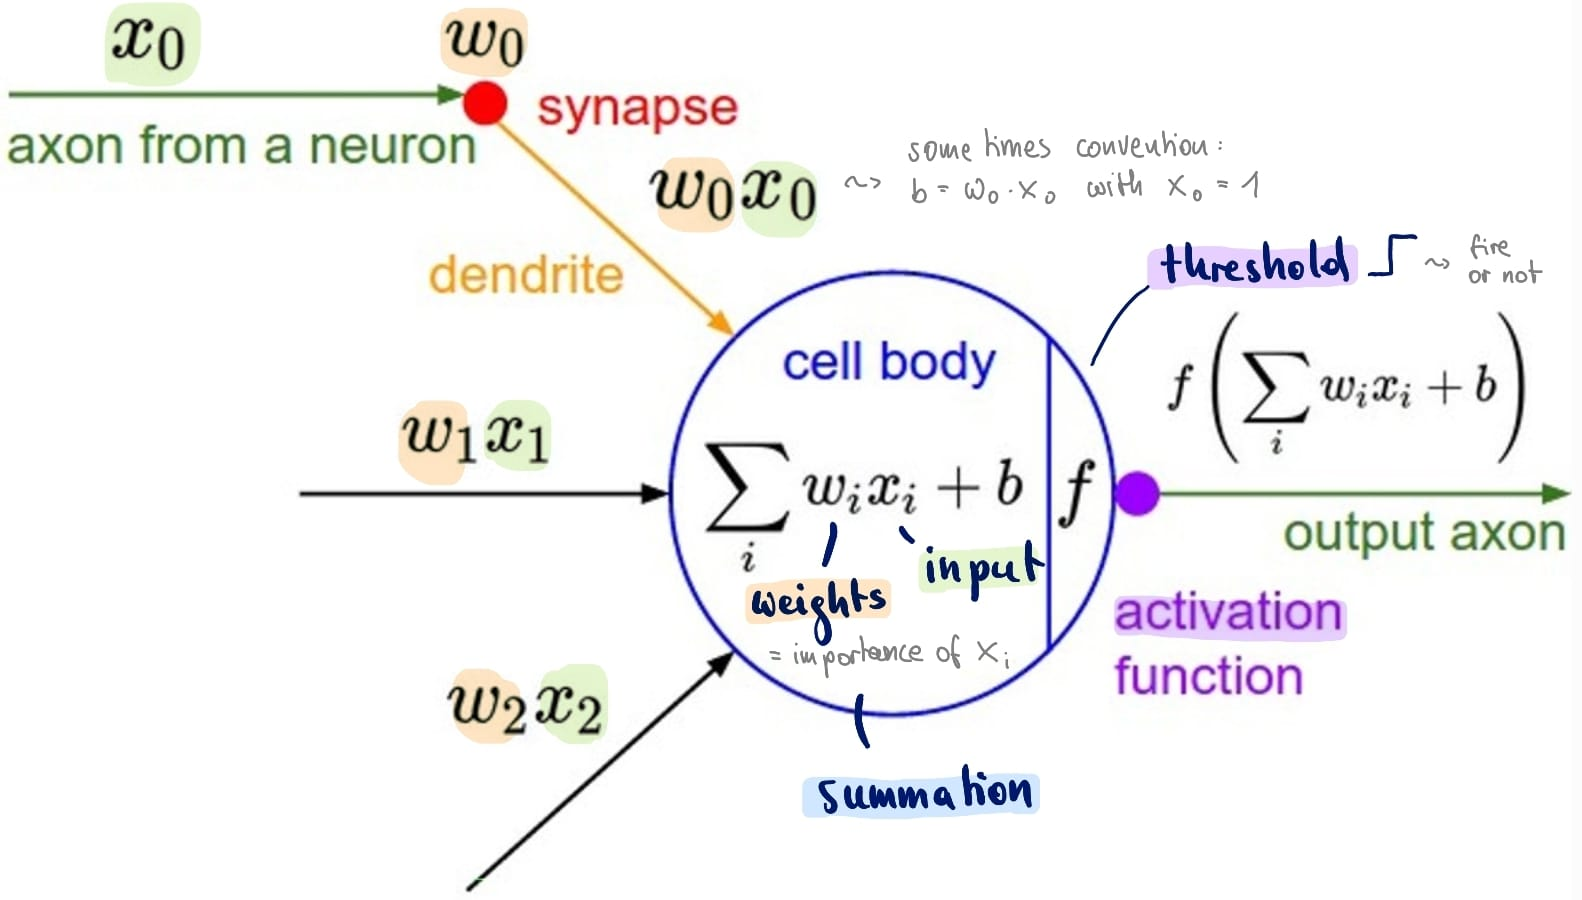
\includegraphics[width=0.6\textwidth]{assets/nn/bg__simple_artificial_neuron.png}
  \caption{Simple artificial neuron (Rosenblatt's perceptron)}
  \label{fig:6_bg_simple_an}
\end{figure}

The \textbf{learning process} of this simple neuron is now the following:
\begin{itemize}
  \item Randomly assign weights $w_i \in [0,1]$
  \item Present inputs from training data $\cv{x}$
  \item Get the output $\cv{y} = f\left(\sum_i w_i x_i\right)$
  \item Compare the calculated output to the training label
  \begin{itemize}
    \item $\rightsquigarrow$ nudge weights to get results towards the desired target output
    \item Repeat until the error is small or the given number of epochs is completed
  \end{itemize}
\end{itemize}

An important detail of the neuron, which needs to be set in the beginning and can't be changed throughout the learning process, is the \textbf{activation function}\sidenote{Activation function}. The choice is free, but here are two typical choices:
\begin{itemize}
  \item Biological neurons use a threshold to decide when to fire. This simple \textbf{step function}\sidenote{Step function} can be imitated by
  \begin{align*}
    f(x) = \begin{array}{ll}
      0,&x<0\\1,&x\geq0
    \end{array}
  \end{align*}
  \item In NNs, the \textbf{sigmoid function}\sidenote{Sigmoid function} (just as in linear regression) is commonly used as the activation function $f$.
  \begin{align*}
    f(x) = sigmoid(x) = \frac{1}{1+e^{-x}}
  \end{align*}
\end{itemize}

Finally, for the simple one-layer perceptrons, we're gonna look at some examples to see what artificial neurons can learn.
\begin{figure}[H]
  \centering
  \begin{subfigure}{\textwidth}
    \centering
    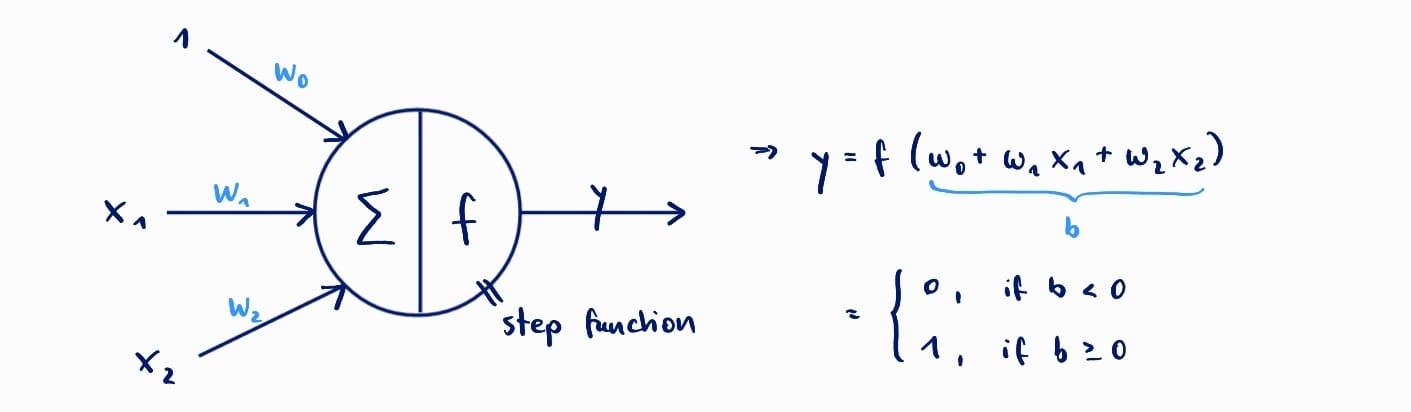
\includegraphics[width=0.75\textwidth]{assets/nn/bg__example_architecture.png}
    \subcaption*{Simple NN architecture}
  \end{subfigure}

  \vspace*{0.5cm}
  \begin{subfigure}{\textwidth}
    \centering\sidenote{AND- and OR-problem}
    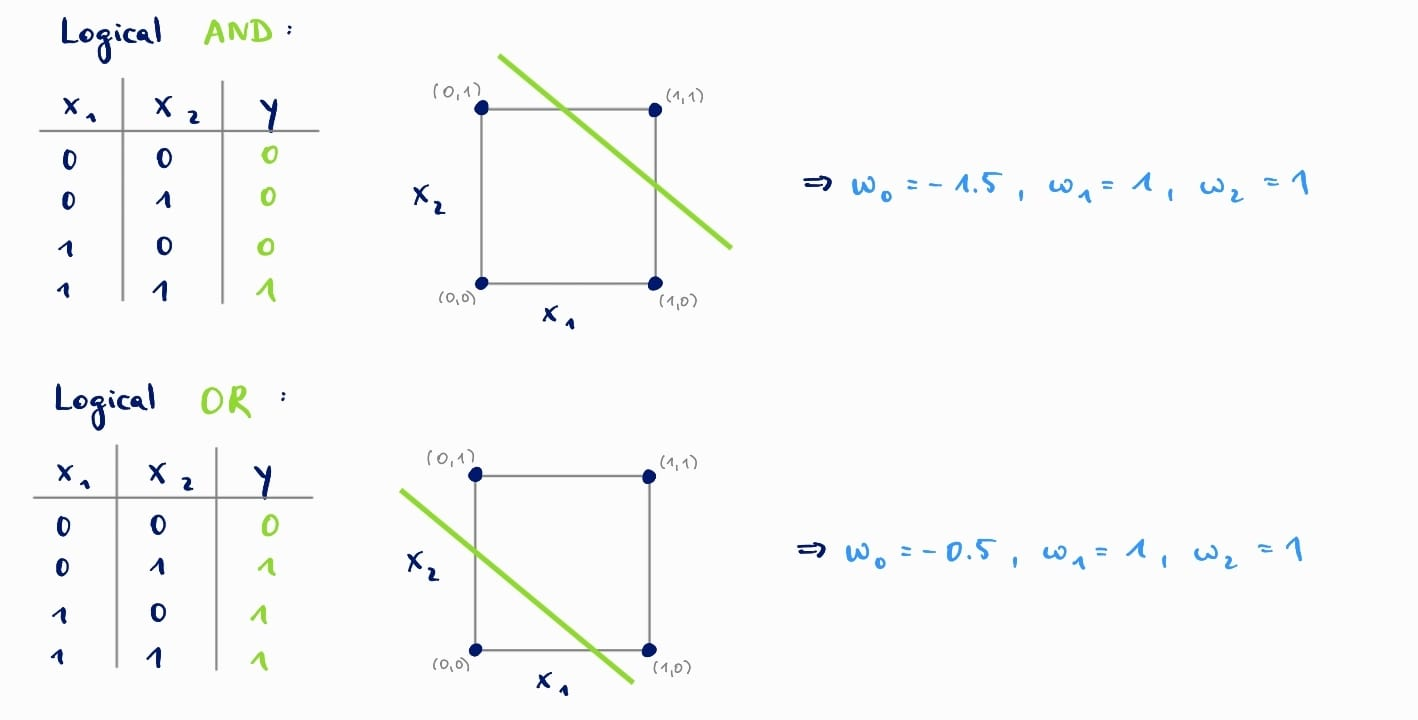
\includegraphics[width=0.75\textwidth]{assets/nn/bg__example_or_and.png}
    \subcaption*{Learnable problems}
  \end{subfigure}

  \vspace*{0.5cm}
  \begin{subfigure}{\textwidth}
    \centering\sidenote{XOR-problem}
    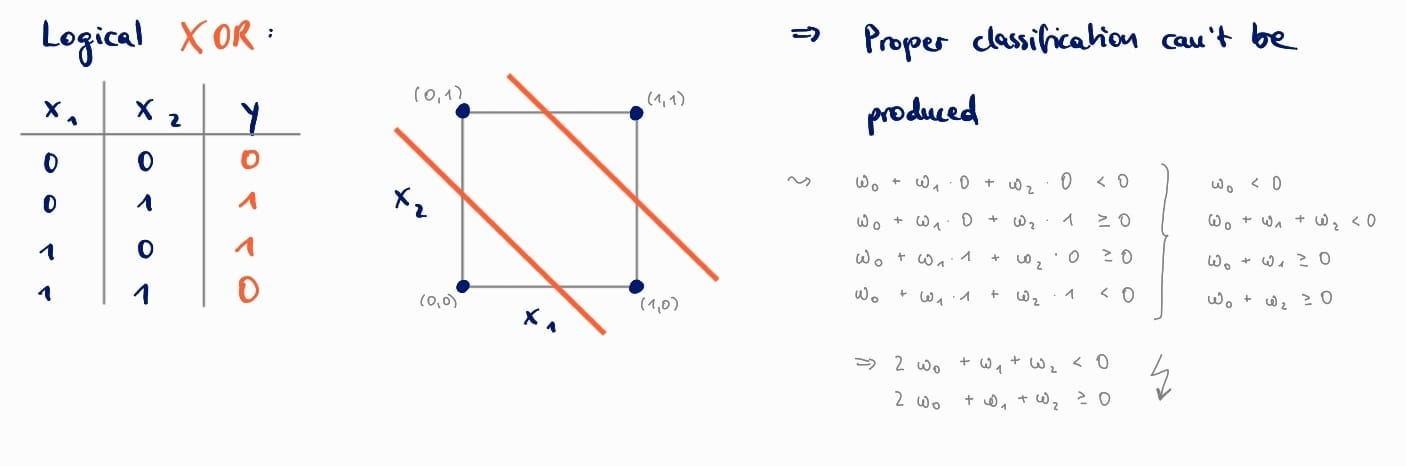
\includegraphics[width=0.75\textwidth]{assets/nn/bg__example_xor.png}
    \subcaption*{Not-learnable problem}
  \end{subfigure}

  \caption{One-layer perceptron: Binary classification examples}
  \label{fig:6_bg_learnable_example}
\end{figure}

The "XOR" example shows the limitations of single-layer perceptrons:
\begin{itemize}
  \item Only a limited set of functions can be represented (e.g. even simple XOR not expressable)
  \item Decision boundaries must be hyperplanes (no non-linearity representable)
  \item Can only perfectly separate linearly separable data
\end{itemize}

